\section{Addressing Overfitting}

\subsection{Dropout Experiment}

\subsubsection{Recorded Values}
\begin{itemize}
    \item Training accuracy: \textbf{99.39\%}
    \item Validation accuracy: \textbf{98.31\%}
    \item Dropout rate: \textbf{0.3 (30\%)}
\end{itemize}

\begin{figure}[h]
    \centering
    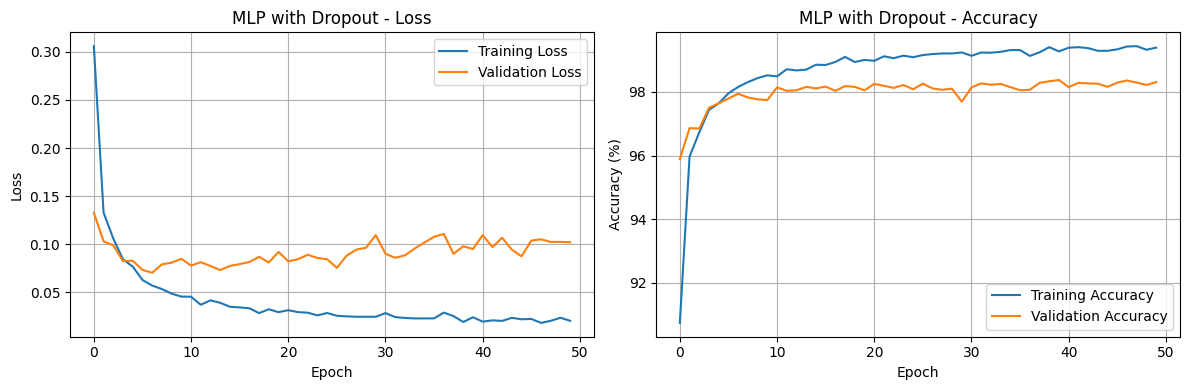
\includegraphics[width=0.8\linewidth]{section2/dropout.png}
    \caption{Training and validation curves for MLP with Dropout (rate=0.3)}
    \label{fig:dropout}
\end{figure}

\subsubsection{Question 2.1: Did dropout help reduce overfitting?}

Yes, dropout significantly reduced overfitting. Validation accuracy improved from 97.74\% (baseline) to 98.31\% (dropout), while training accuracy decreased slightly from 99.79\% to 99.39\%. The gap between training and validation accuracy shrank from 2.1\% to 1.1\%, demonstrating better generalization. 

The loss curves show much less divergence compared to the baseline---validation loss remained stable around 0.08--0.10 throughout training, rather than increasing to 0.19 as observed in the baseline model. This indicates the model learned more robust features instead of memorizing training data.

\subsubsection{Comparison with Baseline}
\begin{table}[h]
\centering
\begin{tabular}{|l|c|c|c|}
\hline
\textbf{Model} & \textbf{Train Acc} & \textbf{Val Acc} & \textbf{Train-Val Gap} \\ \hline
Baseline       & 99.79\%            & 97.74\%          & 2.05\%                 \\ \hline
Dropout        & 99.39\%            & 98.31\%          & 1.08\%                 \\ \hline
\end{tabular}
\caption{Comparison between Baseline and Dropout models}
\label{tab:dropout-comparison}
\end{table}

\subsection{Early Stopping Experiment}

\subsubsection{Recorded Values}
\begin{itemize}
    \item Final epoch: \textbf{11}
    \item Training accuracy: \textbf{99.56\%}
    \item Validation accuracy: \textbf{97.90\%}
    \item Patience: \textbf{5 epochs}
\end{itemize}

\begin{figure}[h]
    \centering
    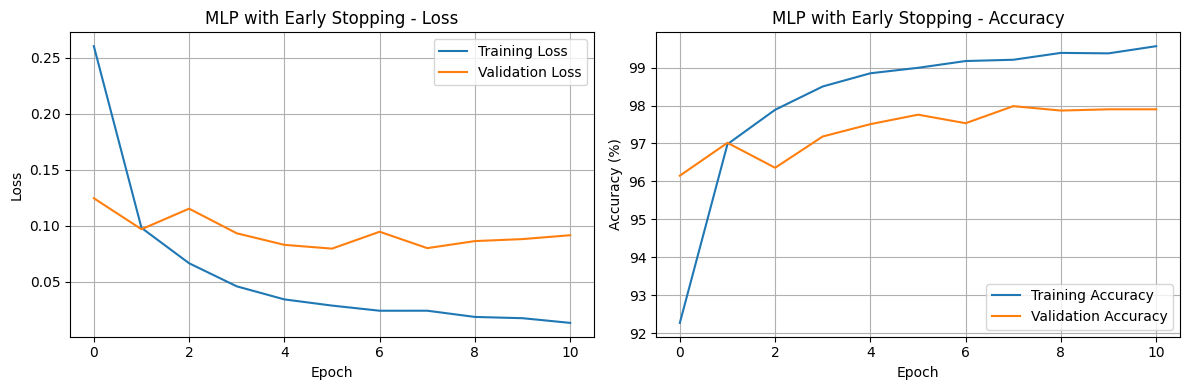
\includegraphics[width=0.8\linewidth]{section2/early_stopping.png}
    \caption{Training and validation curves for MLP with Early Stopping (patience=5)}
    \label{fig:early-stopping}
\end{figure}

\subsubsection{Question 2.2: How did early stopping affect performance?}

Early stopping achieved slightly better validation accuracy (97.90\% vs 97.74\%) compared to the baseline, while training for only 11 epochs instead of 50---a 78\% reduction in training time. This demonstrates that the baseline model was over-training: continuing to train beyond epoch 11 did not improve validation performance and actually led to increased overfitting.

Early stopping efficiently prevented overfitting by monitoring validation loss and stopping training when it plateaued. The validation loss reached approximately 0.09 by epoch 6 and showed no improvement for 5 consecutive epochs, triggering the early stopping mechanism at epoch 11.

\subsubsection{Efficiency Analysis}
\begin{table}[h]
\centering
\begin{tabular}{|l|c|c|c|c|}
\hline
\textbf{Model} & \textbf{Epochs} & \textbf{Train Acc} & \textbf{Val Acc} & \textbf{Efficiency} \\ \hline
Baseline       & 50              & 99.79\%            & 97.74\%          & ---                 \\ \hline
Early Stopping & 11              & 99.56\%            & 97.90\%          & 78\% faster         \\ \hline
\end{tabular}
\caption{Efficiency comparison: Early Stopping vs Baseline}
\label{tab:early-stopping-comparison}
\end{table}

\subsection{Regularization Comparison}

\begin{table}[h]
\centering
\begin{tabular}{|l|c|c|}
\hline
\textbf{Method}        & \textbf{Val Accuracy} & \textbf{Evidence of Overfitting} \\ \hline
Baseline               & 97.74\%               & Yes                              \\ \hline
Dropout                & 98.31\%               & No                               \\ \hline
Early Stopping         & 97.90\%               & No                               \\ \hline
\end{tabular}
\caption{Comparison of regularization techniques for addressing overfitting}
\label{tab:regularization-comparison}
\end{table}

\subsubsection{Overfitting Evidence Analysis}
\begin{itemize}
    \item \textbf{Baseline}: Yes---loss curves diverge significantly after epoch 10, with validation loss increasing from 0.09 to 0.19 while training loss approaches zero. Train-val gap of 2.1\%.
    
    \item \textbf{Dropout}: No---loss curves remain parallel throughout training, with validation loss stable around 0.08--0.10. Reduced train-val gap of 1.1\% indicates better generalization.
    
    \item \textbf{Early Stopping}: No---training stopped at epoch 11 before severe overfitting occurred. Validation loss plateaued at 0.09, and the mechanism prevented further memorization of training data.
\end{itemize}

\subsection{Conclusion}

Both regularization techniques successfully addressed the overfitting problem observed in the baseline model:

\begin{itemize}
    \item \textbf{Dropout} improved validation accuracy by 0.57\% while reducing the train-val gap by half, demonstrating that forcing the network to learn redundant representations leads to better generalization.
    
    \item \textbf{Early stopping} achieved similar validation performance (0.16\% improvement) with 78\% fewer training epochs, proving that the baseline was over-training and that optimal performance can be achieved earlier in the training process.
\end{itemize}

The dropout approach yielded the highest validation accuracy (98.31\%), making it the most effective regularization technique for this task. However, early stopping offers a compelling trade-off between performance and computational efficiency.